\subsection{Financial Models for Option Pricing}
\label{sec:financial_models}

To price financial derivatives, it is necessary to specify a model for the stochastic evolution of the underlying asset. While real markets are driven by complex, often non-stationary dynamics, simplified continuous-time models provide a tractable foundation for pricing and risk management. We begin with the classical Black--Scholes model, which admits a closed-form solution and thus serves as a natural benchmark for evaluating Monte Carlo and differential machine learning (MCDML) approaches.

\subsubsection{Black-Scholes} \label{sec:black-scholes}

In the BS framework, consider the price of a non-dividend paying asset that follows a Geometric Brownian Motion (GBM):
\begin{align}
    dS_t = \mu S_t dt + \sigma S_t dW_t, \label{eq:BS_stock}
\end{align}
where $\mu$ is the drift, $\sigma>0$ is the volatility and $W_t$ is standard Brownian motion under the measure $\mathbb{P}$.

The analytical solution to the Stochastic Differential Equation (SDE) above is,
\begin{align*}
    S_t = S_0 \exp\left( \left(\mu - \frac{\sigma^2}{2}\right)t + \sigma W_t \right).
\end{align*}
which implies that the stock price $S_T$ is lognormally distributed, 
\begin{align*}
    S_T = S_0 \exp\left( \left(\mu - \frac{\sigma^2}{2}\right)T + \sigma \sqrt{T} Z \right), \quad Z \sim N(0,1).
\end{align*}

Under the risk-neutral measure~$\mathbb{Q}$, the drift $\mu$ is replaced by the risk-free rate~$r$, and the time-$0$ price of a European call option with strike~$K$ and maturity~$T$ is
\begin{align}
    C_0 = e^{-rT}\,\mathbb{E}^{\mathbb{Q}}\!\left[\max(S_T - K,0)\right].
    \label{eq:bs_price}
\end{align}
This expectation admits the closed-form Black--Scholes formula, but it also provides a natural Monte Carlo estimator that generalizes to models without analytic solutions. Consequently, we will use the BS model as a benchmark for assessing the accuracy of MCDML in both pricing and Greek estimation.

\subsubsection{Bates} \label{sec:bates}

While the BS model serves as a benchmark for assessing the validity of MCDML method as a pricing and Greek approximator, it is easily simulated using regular MC. To properly assess the performance and potential of MCDML we need a model that requires full path simulation and can benefit from different discretization schemes and variance reduction techniques. For this purpose, we implement a version of the \textcite{batesJumpsStochasticVolatility1996} model\footnote{Technically, the European Call type options do have a semi-analytical solution, using the underlying characteristic function through a Fourier price transform.}. It is a combination of the jump diffusion process mixture model in \textcite{mertonOptionPricingWhen1976} and the \textcite{hestonClosedFormSolutionOptions1993} stochastic volatility model. This setting allow volatility clustering, leptokurtic returns and skewness, and volatility smiles - all empirical features the BS model cannot capture. The discontinuity inherent in jump processes provides an additional challenge for Greek estimation which we will cover later. Originally introduced for Deutsche Mark options, the dynamics are described by the following set of SDEs under the risk-neutral measure~$\mathbb{Q}$:
\begin{align}
    \frac{d S_t}{S_t} &= (r - \lambda \bar{k})dt + \sqrt{v_t}dW_t^S + k dN_t, \label{eq:bates_stock} \\
    dN_t &= \lambda dt + dJ_t, \\
    \frac{d S_t}{S_t} &= (r - \lambda \bar{k})dt + \sqrt{v_t}dW_t^S + dJ_t, \\
    dv_t &= \kappa(\theta - v_t)dt + \sigma\sqrt{v_t}dW_t^v, \label{eq:bates_stoch_vol} \\
    %\text{corr}(dW_t^S, dW_t^v) &= \rho,
    dW_t^S dW_t^v &= \rho dt, \label{eq:corr_brownian}
\end{align}
where $N_t$ is a Poisson process with intensity $\lambda$, $k$ is the random jump size with mean $\bar{k}$ (subtracted to keep the discounted price a martingale), $v_t$ is the instantaneous variance, $\kappa > 0$ is the rate of mean reversion, $\theta >0 $ is the long-term variance, $\sigma$ is the volatility of volatility, and $\rho$ is the correlation between the asset price and its variance. It follows that \eqref{eq:bates_stock} is BS stock price dynamics augmented with a jump component, with expected relative jump-size $\bar{k} = \mathbb{E}[e^Y-1]=e^{\mu_J + \frac{1}{2}\delta_J^2}-1$ where $Y \sim \mathcal{N}(\mu_J, \delta^2_J)$ i.e. log-normal jump-sizes, while \eqref{eq:bates_stoch_vol} is the Heston variance process, following a Cox-Ingersoll-Ross (cite) (CIR) (or mean-reverting square root process) ensuring positivity as long as the Feller condition $2\kappa \theta > \sigma^2$ holds. Lastly, \eqref{eq:corr_brownian} allows for correlation between the two Brownian motions, which is essential to capture the leverage effect observed in real markets.

% Maybe change, and use this 
% \begin{figure}[htbp]
%     \centering
%     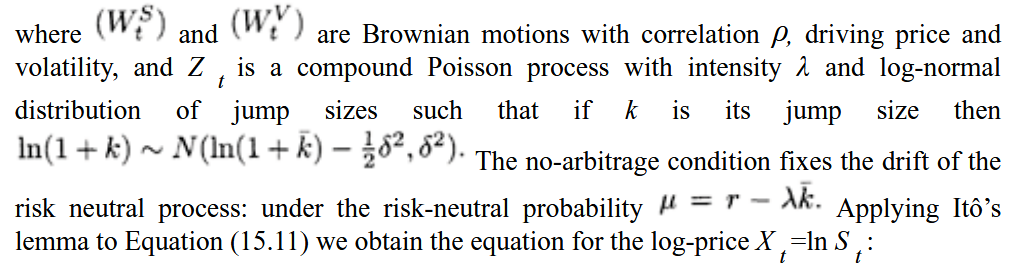
\includegraphics[width=1\textwidth]{image3.png}
%     \caption{image3}
%     \label{fig:image3}
% \end{figure}

Following \textcite{contFinancialModellingJump2003}, applying Itô's lemma to \eqref{eq:bates_stock} yields the SDE for the log-price process,
\begin{align}
    dX_t = \left(r - \lambda \bar{k} - \frac{1}{2}v_t\right)dt + \sqrt{v_t}dW_t^S + d \tilde{J}, \label{eq:bates_logprice}
\end{align}
where $X_t = \log(S_t)$ and $\tilde{J} = \sum_{i=1}^{N_t} Y_i$ is a compound Poisson process with normally distributed jump sizes $Y_i \sim \mathcal{N}(\mu_J, \delta_J^2)$. 

% Now, for European call options, given the characteristic function of the log-price process, we can price options using Fourier transform methods as in \textcite{carrOptionValuationAlternative1999} and \textcite{leeOptionPricingFourier2004}. However, to fully leverage the MCDML framework, we will instead rely on Monte Carlo simulation to estimate option prices and Greeks, as detailed in the next section. 

\subsubsection{Greeks}

In addition to pricing, a key aspect of option risk management involves computing sensitivities of the option price to various model parameters, commonly referred to as the "Greeks". The primary Greeks include Delta ($\Delta$), Gamma ($\Gamma$), Vega ($\nu$), Theta ($\Theta$), and Rho ($\rho$). 

WRITE SOMETHING REAL ABOUT WHY THESE ARE IMPORTANT FOR HEDGING ETC. 
